\chapter{Vibraciones Estocásticas}

\section{Proceso Estocástico}
Una \textcolor{red}{variable aleatoria} $X$ toma una ``realización'' (valor), no hay un efecto del tiempo. \\

Ejemplos de variables aleatorias:
\begin{itemize}
    \item Período de retorno (``ocurrencia'') de un terremoto % $ > M_w8.5$
    \item Módulo de Young de un material (Hormigón: $E_c$)
    \item Resistencia característica (Acero: $F_y$)
    \item Geometría
    \item Intensidad de un terremoto en un sitio específico.
\end{itemize}

Un \textcolor{red}{proceso estocástico} (p.e.) es una colección de variables aleatorias para cada $t \in T$. Para los casos prácticos de este curso, la indexación $t$ puede ser el tiempo, por lo que la colección es secuencial. Además, un p.e. puede ser continuo (imposible de hacer en computador) o discreto (conjunto/arreglo/vector). \\
\begin{align*} 
    \Longrightarrow \{X(t): t \in T\} =\{X(t_1), X(t_2), ..., X(t_m)\}
\end{align*}

Una realización de un proceso estocástico corresponde a la realización de todas las variables aleatorias de su colección. \\

Realización 1: 
\begin{figure}[H]
\centering
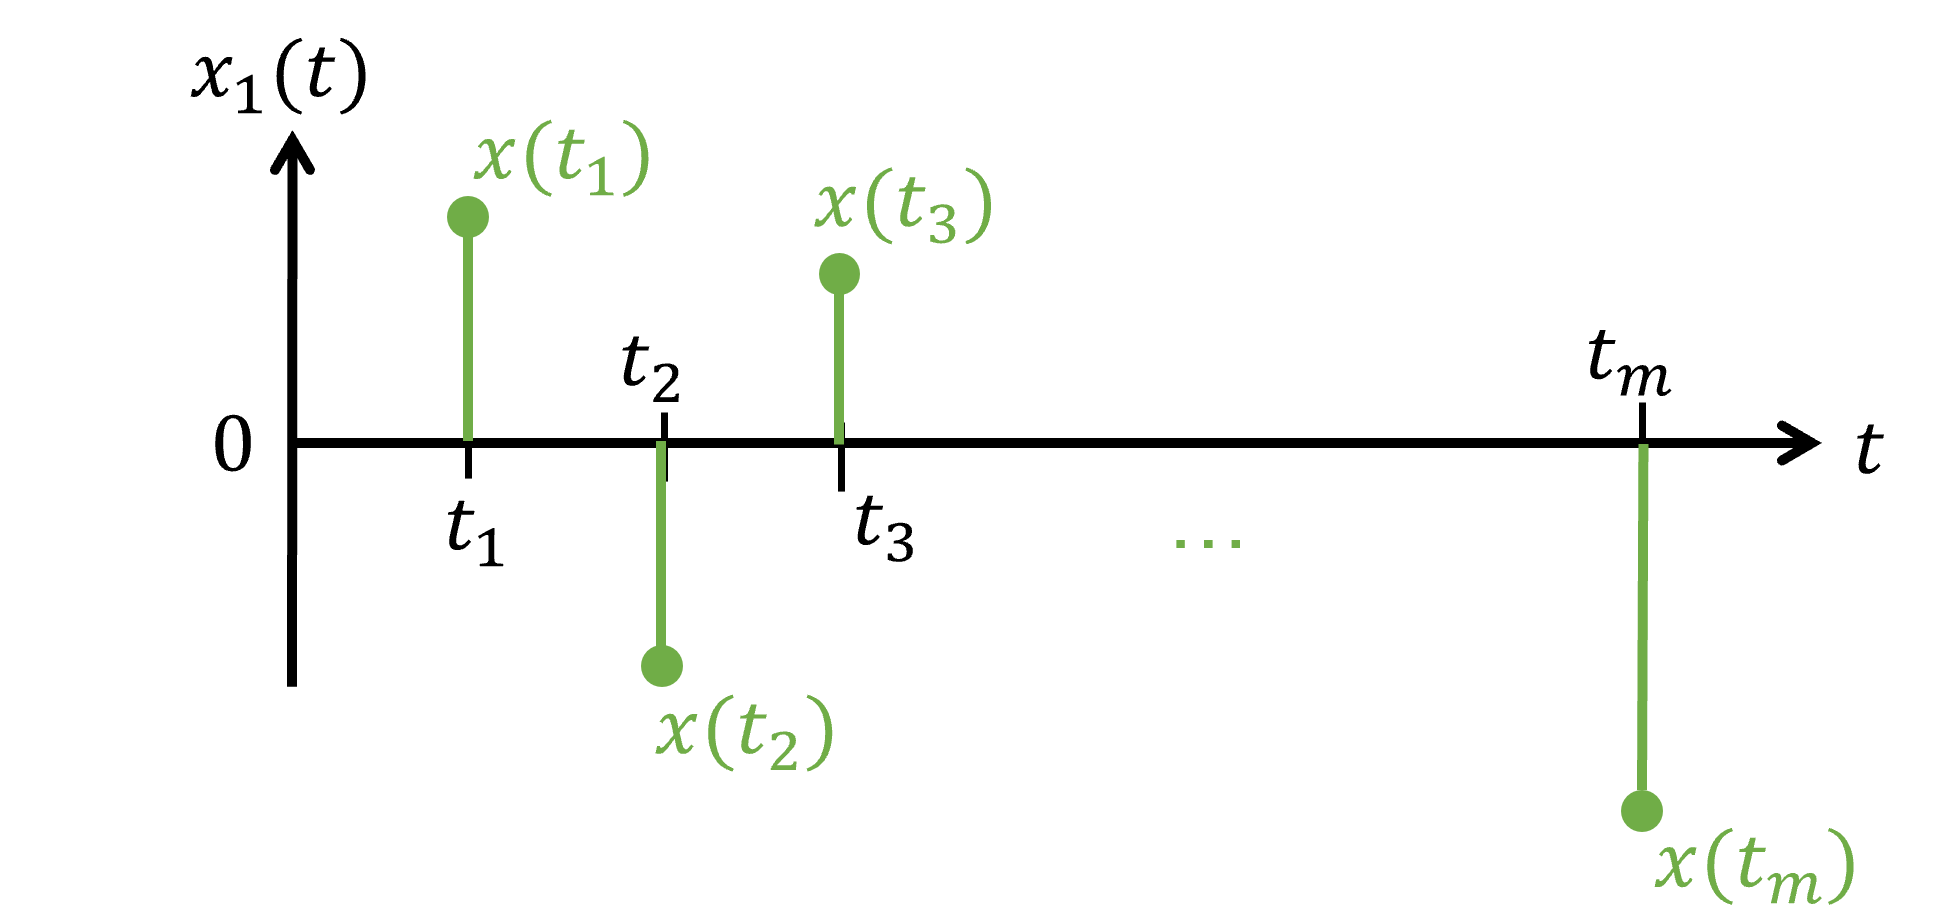
\includegraphics[scale=0.7]{Figuras/pe.png}
\end{figure}

Realización 2: 
\begin{figure}[H]
\centering
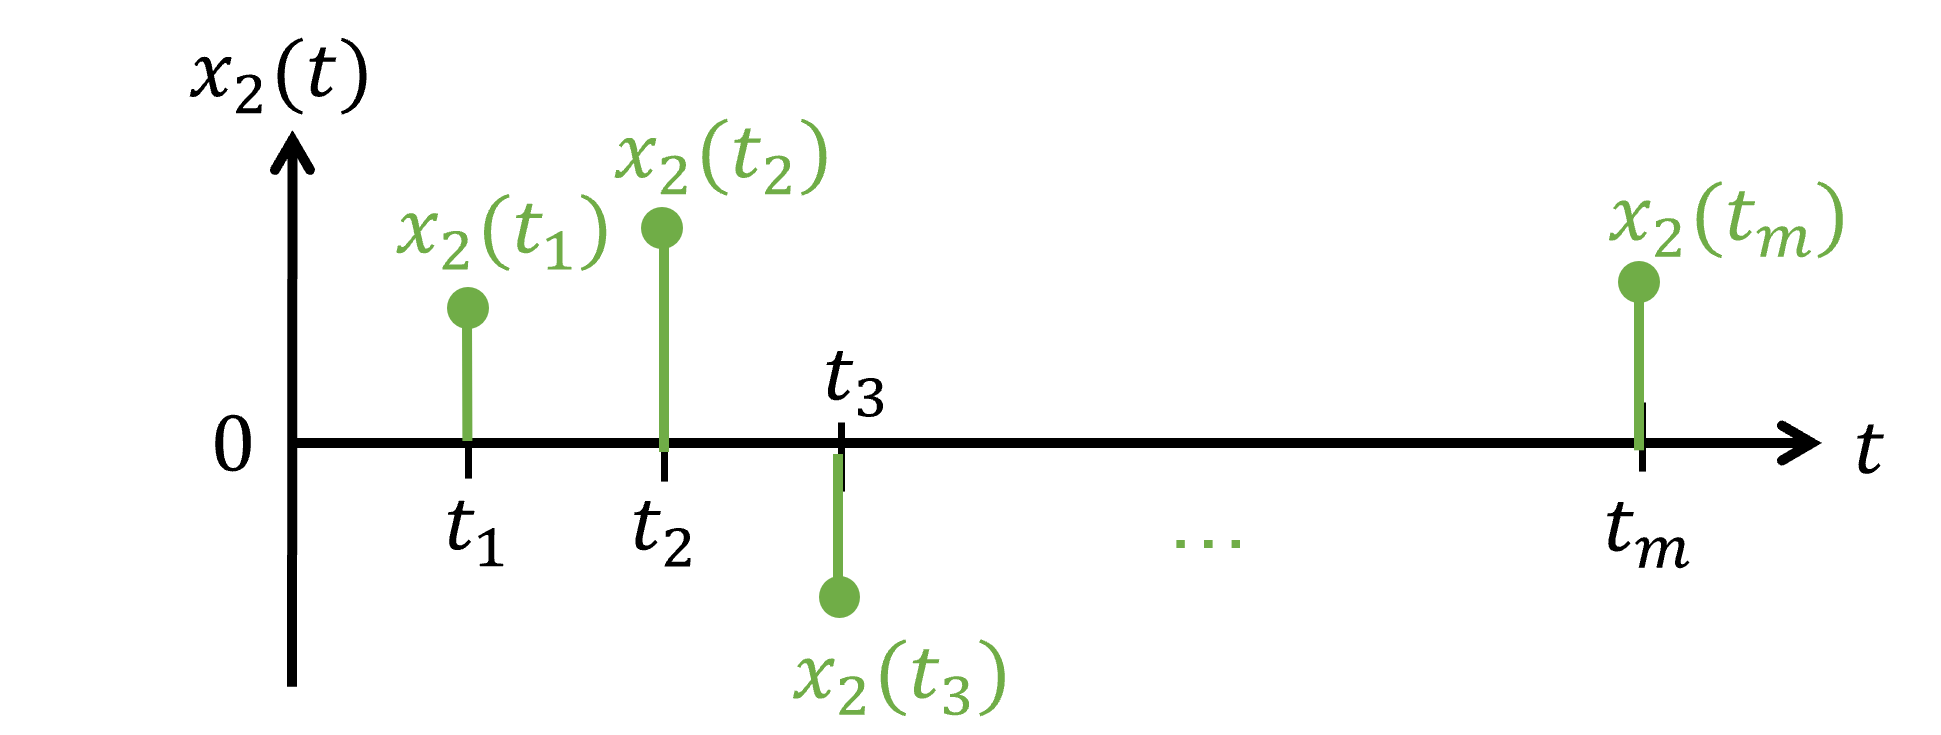
\includegraphics[scale=0.7]{Figuras/pe2.png}
\end{figure}

\par Ejemplos de p.e. para aplicación en ingeniería estructural y sísmica:
\begin{itemize}
    \item Vibraciones aleatorias
    \item Registro de aceleración de un terremoto
    \item Presión del viento
    \item Carga de tráfico un puente
\end{itemize}

\par Existen 2 formas de describir un p.e. $\{X(t)$, $t\in T\}$:
\begin{enumerate}
    \item Función de distribución conjunta (ej: CDF)
    \begin{align*}
        \mathbb{P}[X(t_1)\leq x_1 \cap X(t_2)\leq x_2 \cap ... \cap X(t_m) \leq x_m ] = F_X(x_1,x_2,...,x_m;t_1,t_2,...,t_m)
    \end{align*}
    \item Momentos estocásticos $\Longrightarrow$ momentos de 1er y 2do orden
    \begin{itemize}
        \item Media $(m \times 1)$: $$\mu _X(t_i)=\mathbb{E}\{X(t_i)\}$$
        \item Varianza $(m \times 1)$: $$\sigma _X^2(t_i)=\mathbb{E}\{[X(t_i)-\mu_X(t_i)]^2\}$$
        \item Función de auto-correlación $(m \times m)$: $$R_{XX}(t_i,t_j)=\mathbb{E}\{X(t_i)X(t_j)\}$$
        \item Función de auto-covarianza $(m \times m)$: $$\Gamma_{XX}(t_i,t_j)=\mathbb{E}\{[X(t_i)-\mu_X(t_i)][X(t_j)-\mu_X(t_j)]\}$$ $$\Gamma_{XX}(t_i,t_j)=R_{XX}(t_i,t_j)-\mu_X(t_i)\mu_X(t_j)$$
        \item Coeficiente de correlación $(m \times m)$: $$\rho_{XX}(t_i,t_j) = \frac{\Gamma_{XX}(t_i,t_j)}{\sigma_X(t_i)\sigma_X(t_j)}$$ \\

        Notar que: $$\rho_{XX}(t_i, t_i) = 1$$\\
        
        Interpretación: ``medida de independencia lineal entre variables aleatorias''. \\
        \begin{figure}[H]
            \centering
            \subfigure[]{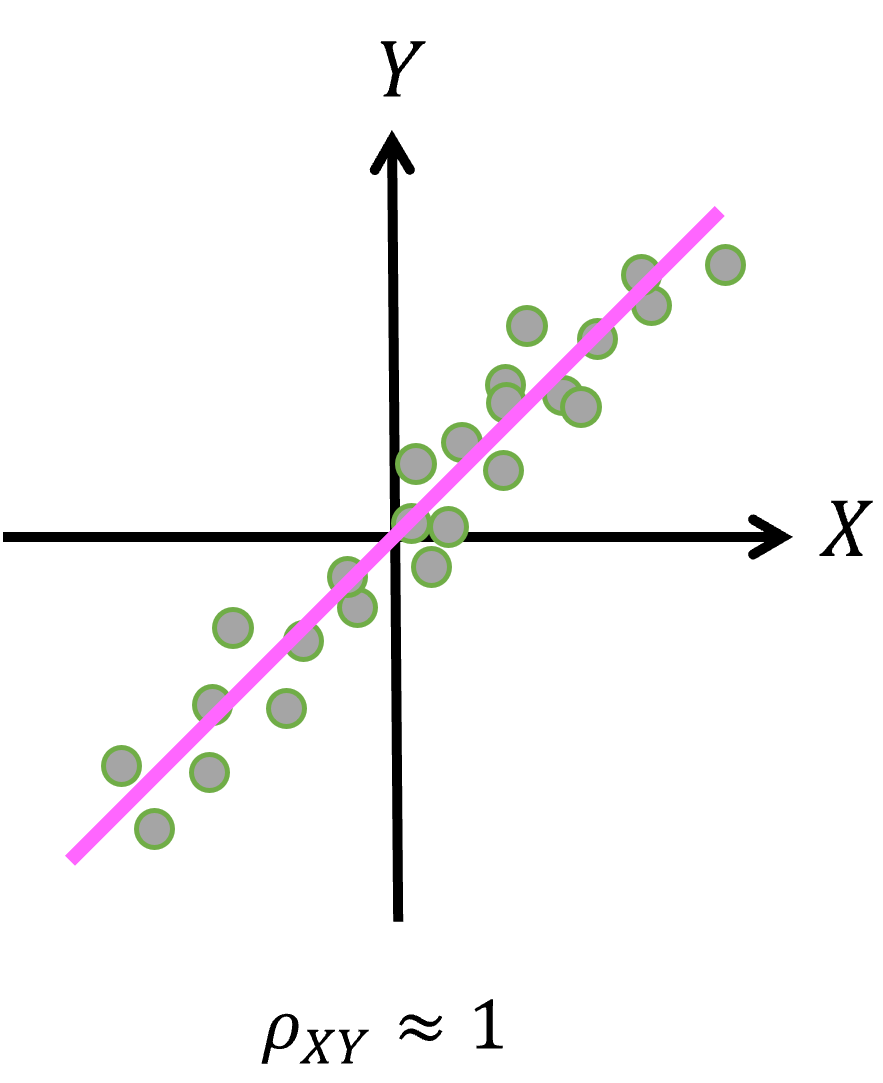
\includegraphics[scale=0.7]{Figuras/rho1.png}}
            \subfigure[]{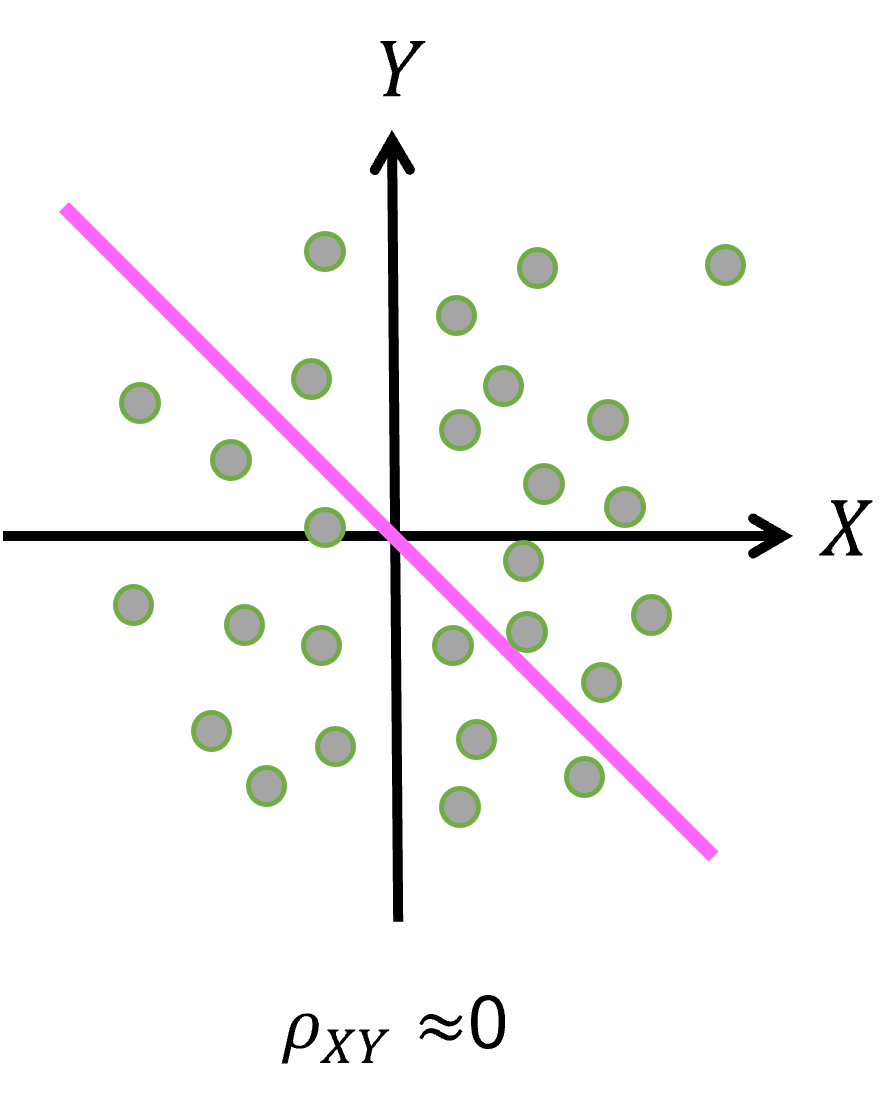
\includegraphics[scale=0.7]{Figuras/rho0.png}}
        \end{figure}
        Notas: \begin{itemize}
            \item $|\rho_{XX}(t_i,t_j)| \leq 1$
            \item Si $\rho_{XX}(t_i,t_j)=0$, $\forall t_i \neq t_j$, entonces el p.e. es un proceso descorrelacionado (por ejemplo: ruido blanco).
        \end{itemize}
    \end{itemize}
\end{enumerate}

En caso de dos procesos estocásticos, $\{X(t)$, $t \in T_X\}$ y $\{Y(t)$, $t \in T_Y\}$ dos procesos estocásticos (ej.: sismo y respuesta estructural):
\begin{itemize}
    \item Función de correlación cruzada: $$R_{XY}(t_i,t_j)=\mathbb{E}\{X(t_i)Y(t_j)\} $$
    \item Función de covarianza cruzada:
    $$\Gamma_{XY}(t_i,t_j) =\mathbb{E}\{ [X(t_i)-\mu_x(t_i)][Y(t_j)-\mu_y(t_j)]\} $$
    $$\Gamma_{XY}(t_i,t_j) = R_{XY}(t_i, t_j)-\mu_X(t_i)\mu_Y(t_j) $$ 
    \item Coeficiente de correlación cruzado: $$\rho_{XY}(t_i,t_j)=\frac{\Gamma_{XY}(t_i,t_j)}{\sigma_X(t_i)\sigma_Y(t_j)} $$
\end{itemize}

% Ej.: p.e. de terremoto (X) y p.e. de respuesta estructural (Y), estos están correlacionados. githu

\section{Clasificación de P.E.}
\begin{enumerate}
    \item \underline{P.E. no estacionario}: La distribución de probabilidad del p.e. depende del tiempo. Las variables aleatorias de la colección no tienen la misma distribución.
    \begin{figure}[H]
    \centering
    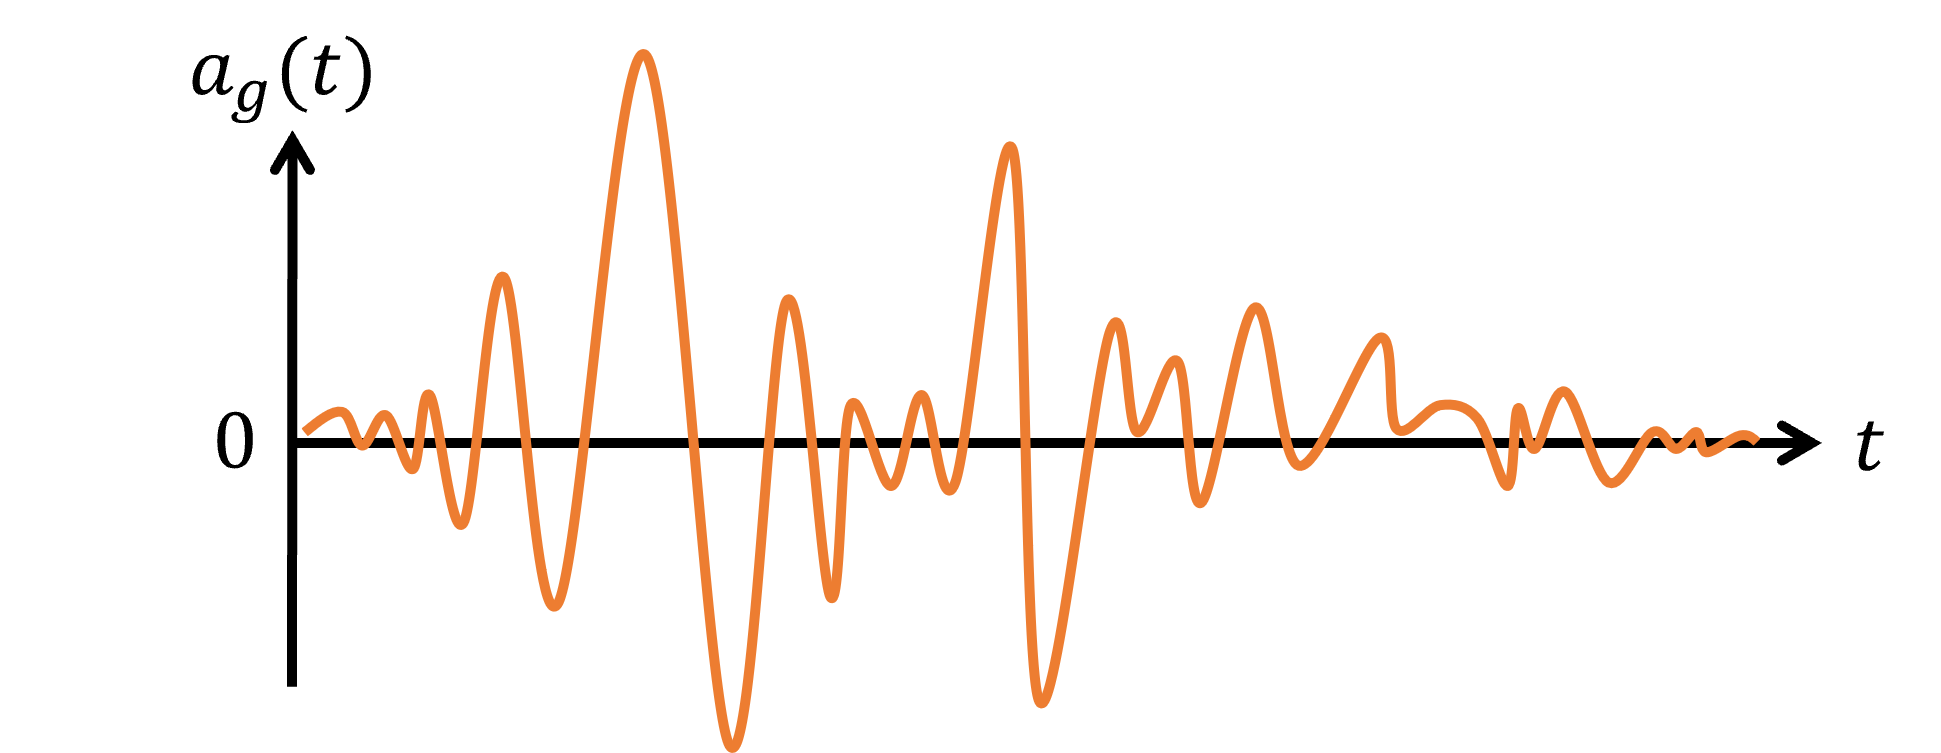
\includegraphics[scale=0.7]{Figuras/penoesatacionario.png}
    \end{figure}
    
    \item \underline{P.E. Estrictamente estacionario}: La distribución de probabilidad del p.e. no cambia con un retraso en el tiempo:
    \begin{equation*}
        F_X(x_1,...,x_m; t_1,...,t_m) = F_X(x_1,...,x_m; \textcolor{brown}{t_1 + \tau,...,t_m + \tau})
    \end{equation*}
    \begin{figure}[H]
    \centering
    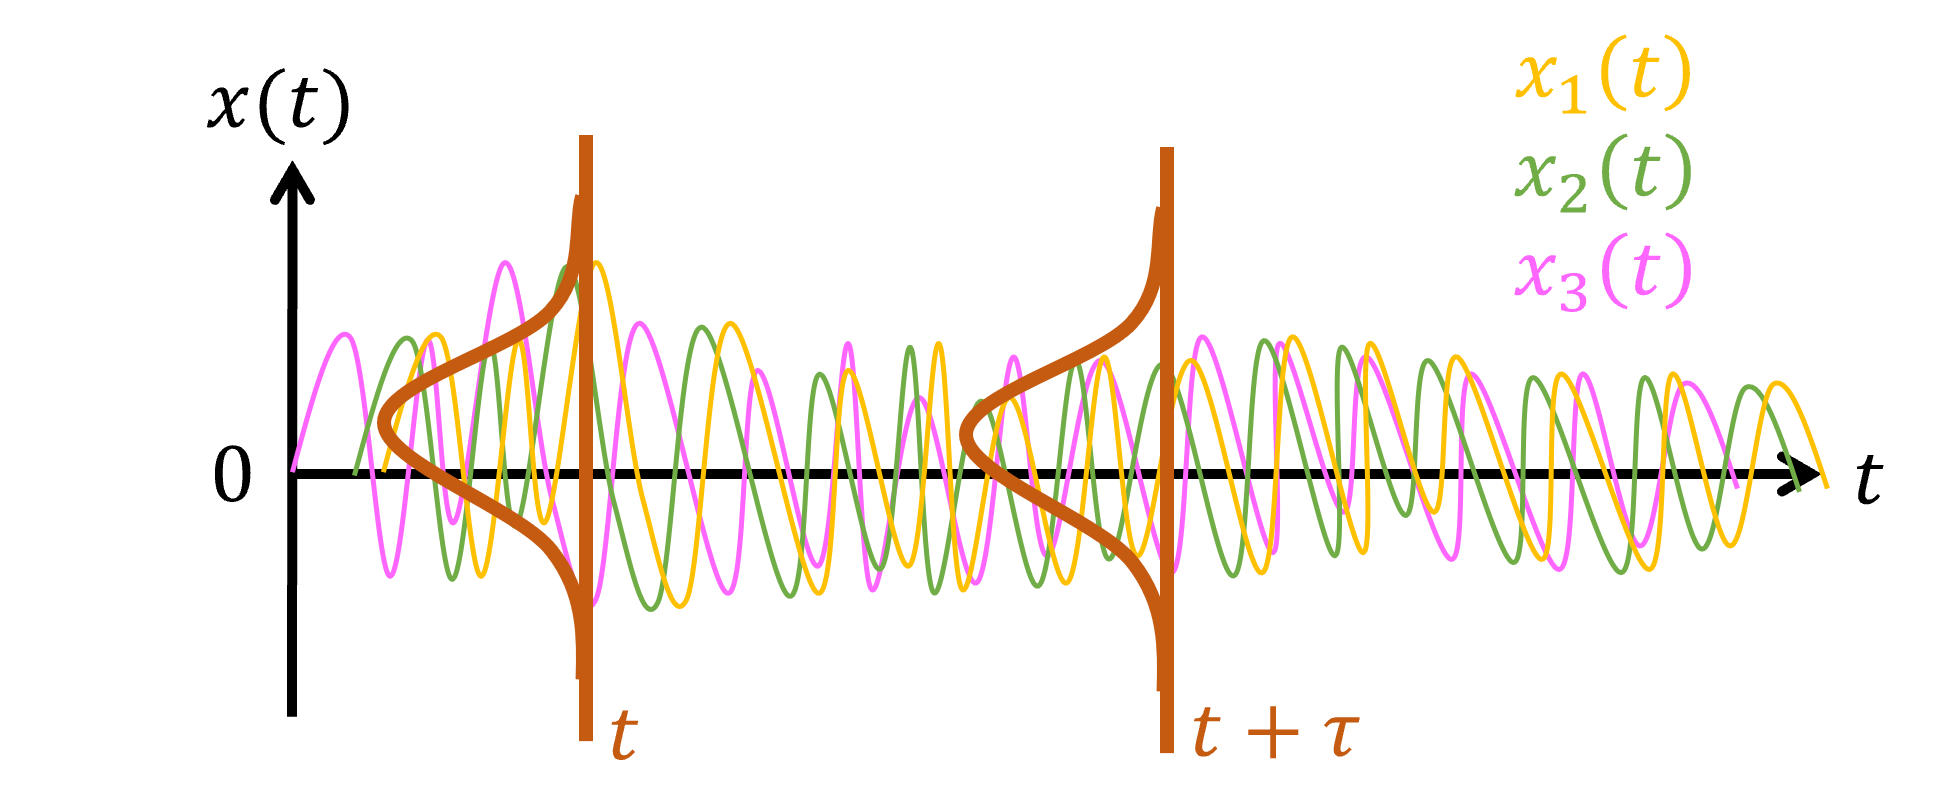
\includegraphics[scale=0.7]{Figuras/peestricto.png}
    \end{figure}
    \item \underline{P.E. Débilmente estacionario}: Estadísticos de 2do orden son finitos y no varían en el tiempo
    \begin{align*}
        &\phantom{\Longrightarrow}\mu_X(t_i)=\mu_X(t_j) = cste, \quad \sigma_X^2(t_i)=\sigma_X^2(t_j)=cste\\
        &\Longrightarrow R_{XX}(t_1,t_2) = R_{XX}(t_2-t_1)
    \end{align*}
\end{enumerate}

\section{P.E. Gaussiano}
Un p.e. $\{X(t)$, $t \in T\}$, se llama un p.e. Gaussiano si, para cada conjunto $\{t_1,t_2,...,t_m\}\in T$, las ``m'' variables aleatorias $X(t_1)$, $X(t_2)$, $...,$ $X(t_m)$ son distribuidas normales multivariadas.
\begin{align*}
    \{X(t), t \in T\}\sim~ N\big(\mu_X,\Gamma_{XX}\big)
\end{align*}
donde $\mu_X$ es el vector de las medias de las variables aleatorias del p.e. y $\Gamma_{XX}$ es la matriz de auto-covarianza. \\

\underline{Notas}:
\begin{itemize}
    \item Un p.e. Gaussiano y débilmente estacionario es estrictamente estacionario.
    \item Un p.e. Gaussiano preserva las transformaciones lineales, y esto es extremadamente útil en los problemas de sistemas lineales que se verán más adelante.
\end{itemize}

\section{Función de Autocorrelación}
Dado $\{X(t), t \in T\}$ un w.s.s., la \emph{función de autocorrelación} $R_{XX}(\tau) = R_X(\tau)$ se define como:
\begin{align*}
    R_{X}(\tau)=\mathbb{E}\{X(t)X(t+\tau)\}
\end{align*}

\underline{Características de $R_X(\tau)$}:
\begin{enumerate}
    \item $R_X(\tau)$ es una función par
    \begin{align*}
        R_X(\tau)=R_X(-\tau)
    \end{align*}
    \item $R_X(\tau)$ debe ser finita. Adicionalmente.:
    \begin{align*}
        |R_X(\tau)|&\leq R_X(0)\\
        \Longrightarrow R_X(0)&=\mathbb{E}\{X^2(t)\}=\sigma^2_X(t)+\mu_X^2(t)
    \end{align*}
    En $\tau=0$, $R_X(0)$ entrega el máximo valor de la media cuadrada del p.e. $\{X(t), t \in T\}$.
    \item $R_X(\tau)$ es una función definida positiva.\\
    $\Longrightarrow$ Para cualquier función $g(t)$, si:
    \begin{align*}
        g(t_1)R_X(t_1-t_2)g(t_2)\geq 0
    \end{align*}
    Por lo tanto, $R_X(\tau)$ es definida positiva siempre.
    \item $R_X(\tau)$ es continua en $\tau$.
\end{enumerate}

\section{Densidad de Poder Espectral (power spectral density, PSD)}
\underline{Definición}: Densidad de poder espectral (PSD) (Teorema de Wiener-Khintchine).\\
\par Sea $X=\{X(t): t\in T\}$ un p.e. w.s.s. (weakly strictly stationary), con función de autocorrelación $R_x(\tau)$. La función de densidad de poder espectral se define como la \emph{transformada de fourier} de la \emph{función de autocorrelación}:
\begin{align*}
    S_X(\omega) &=\mathcal{F}\{R_X(\tau)\}\\
    R_X(\tau) &=\mathcal{F}^{-1}\{S_X(\omega)\}
\end{align*}

\par \underline{Propiedades PSD}:
\begin{enumerate}
    \item Función real
    \item Función simétrica
    \item Definida positiva
    \item Área bajo la curva de $S_X(\omega)$ es igual a $\mathbb{E}\{X^2(t)\} = \sigma^2_X(t) + \mu^2_X(t) = R_X(\tau=0)$
\end{enumerate}
\begin{figure}[H]
\centering
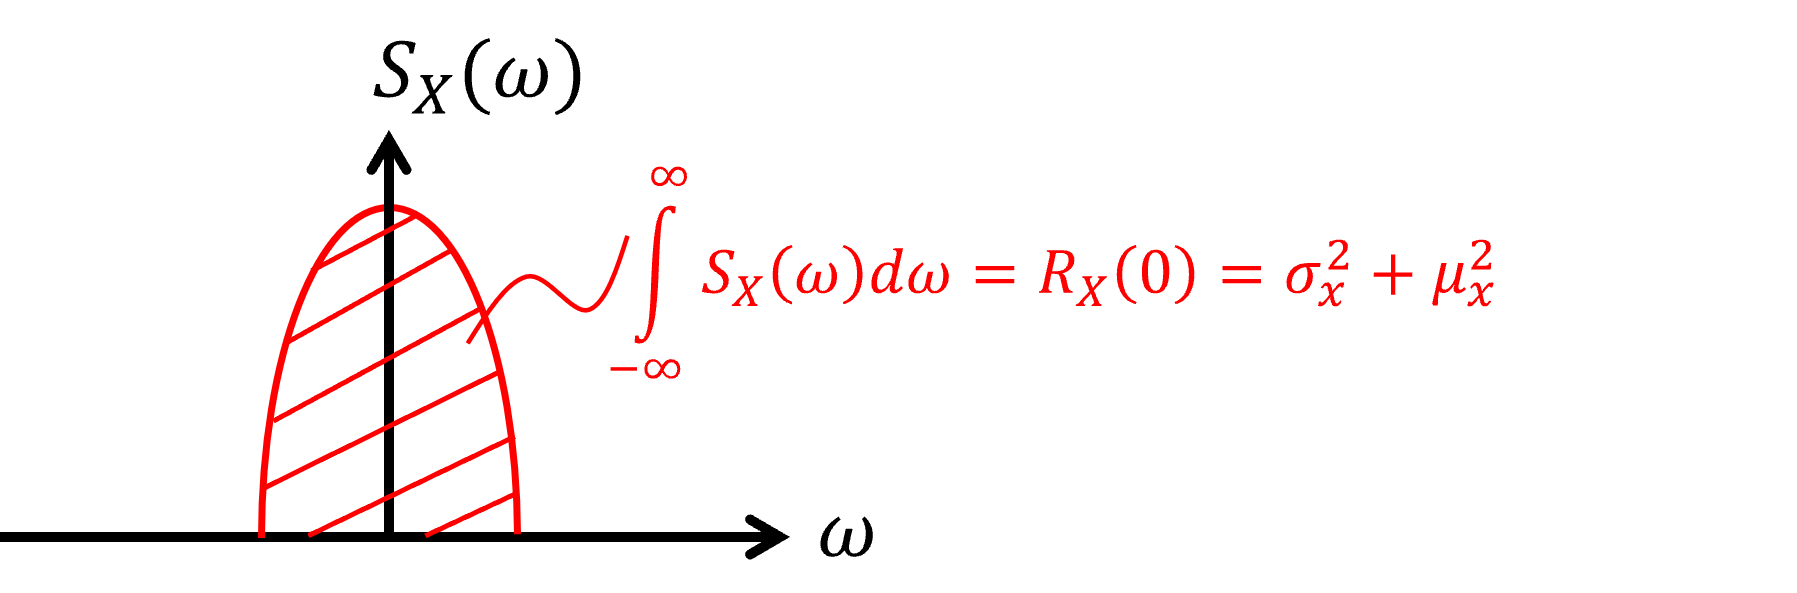
\includegraphics[scale=0.7]{Figuras/PSD.png}
\end{figure}

\section{Ruido blanco}
Sea $X=\{X(t): t\in T\}$ un p.e. w.s.s. Gaussiano, con $\mu_X=0$, $X$ es un ruido blanco si su PSD es constante:
\begin{align*}
    S_X(\omega) &= S_0, \quad \forall \omega \in (-\infty,+\infty)\\
    \Longrightarrow R_X(\tau) &= 2\pi S_0\delta (\tau)
\end{align*}

donde $\delta(\tau)$ es el delta de Dirac.
\begin{figure}[H]
\centering
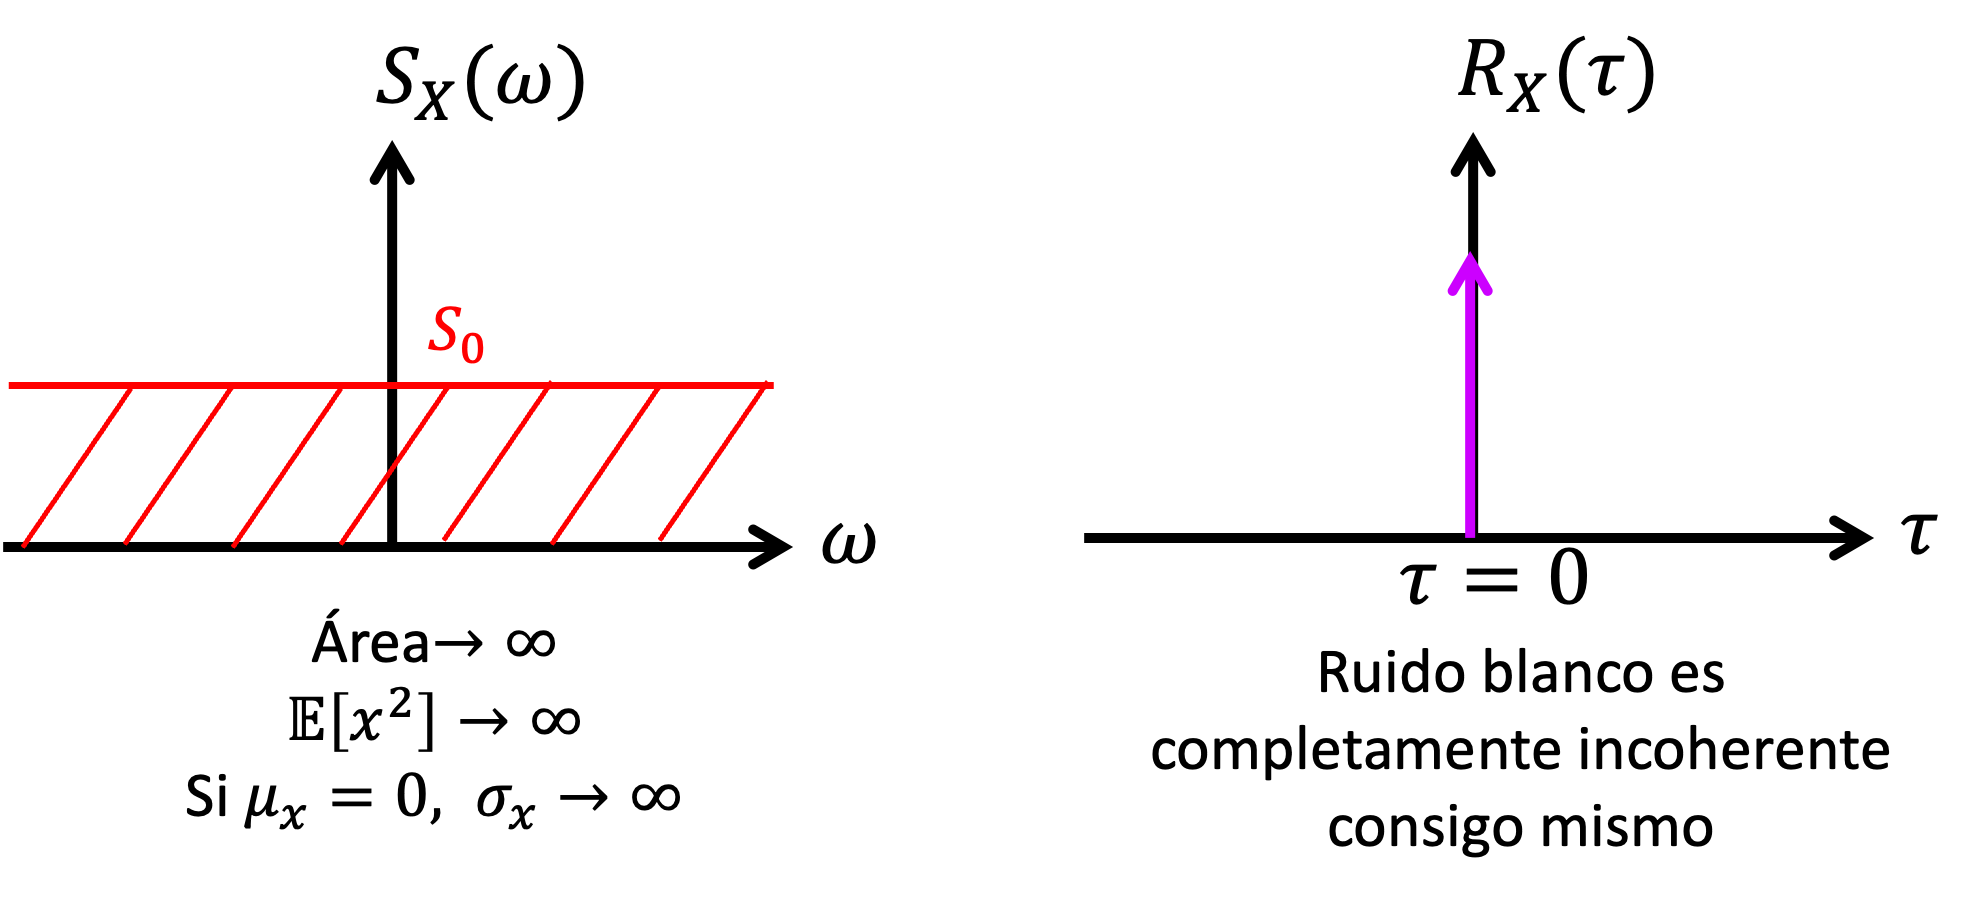
\includegraphics[scale=0.7]{Figuras/ruidoblanco.png}
\end{figure}


\subsection{Ruido blanco de banda limitada (band-limited white noise, BLWN)}
Sea $X$ un p.e., w.s.s., es un \emph{ruido blanco de banda limitada} (BLWN) si:
\begin{align*}
    S_X(\omega) & = \left\{
\begin{array}{ll}
      S_0 & |\omega|\leq \omega_c \\
      0 & |\omega|> \omega_c \\
\end{array} 
\right. \\
    R_X(\tau) & = R(0)\frac{\sin(\omega_c \tau)}{\omega_c \tau}\\
    & = R(0)\text{sinc}(\omega_c \tau)
\end{align*}

\begin{figure}[H]
\centering
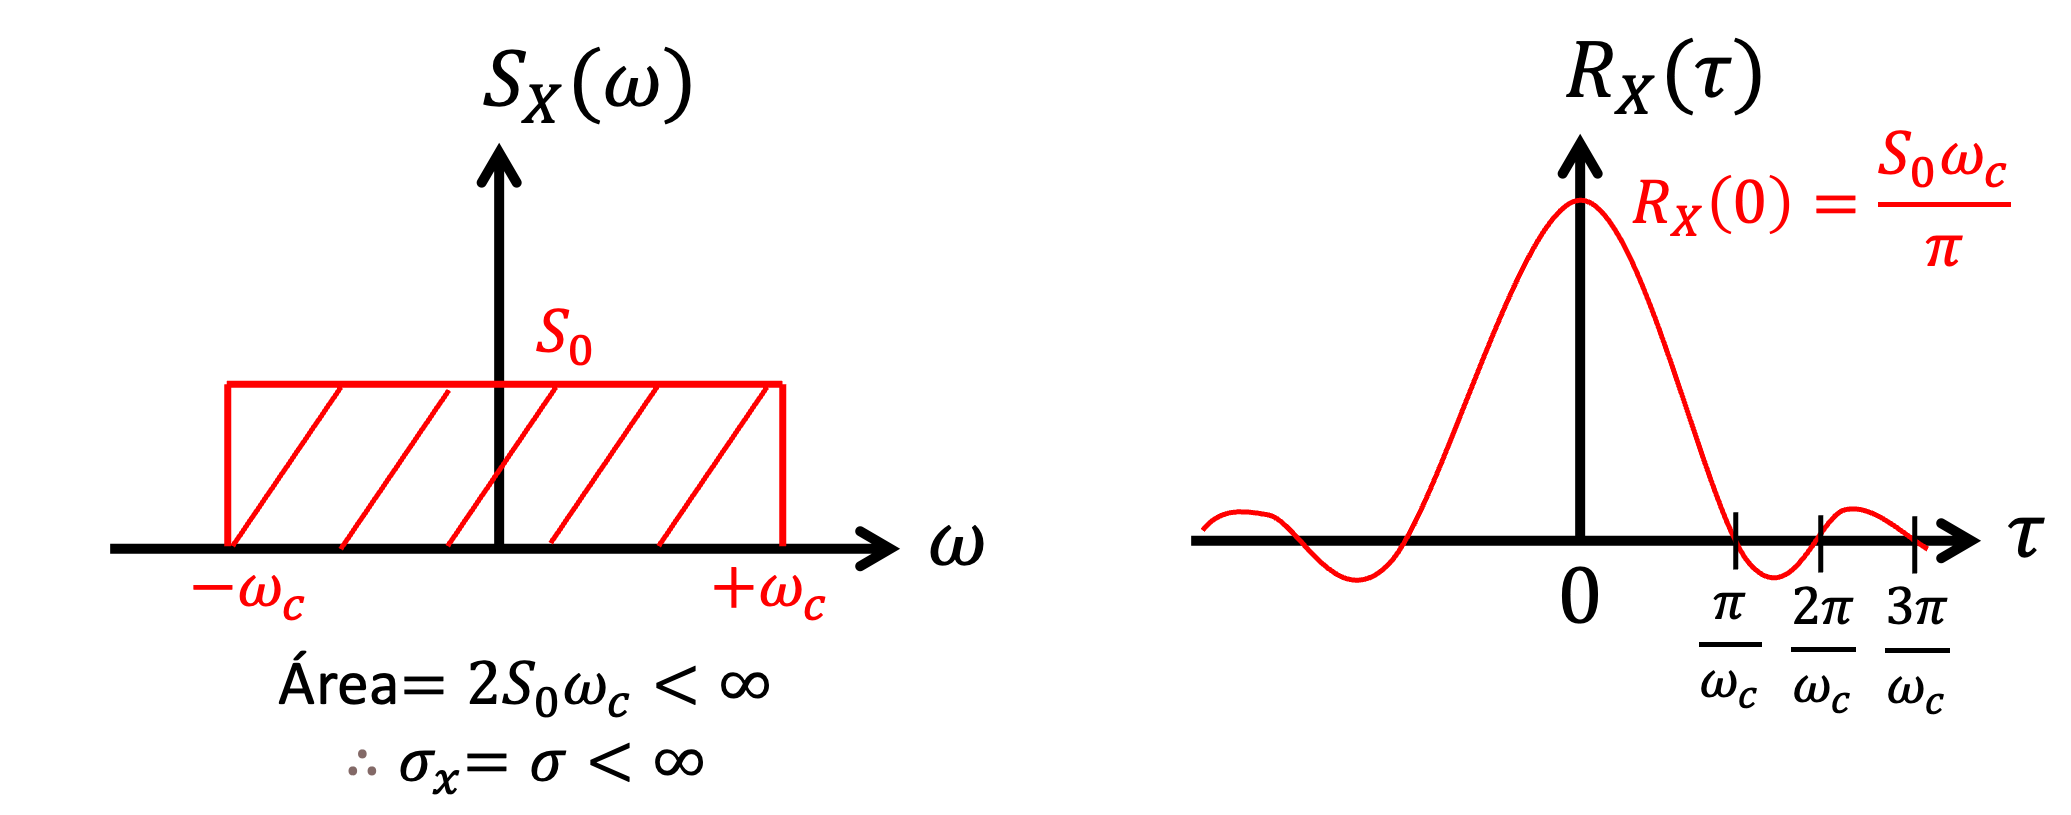
\includegraphics[scale=0.7]{Figuras/BLWN.png}
\end{figure}

Nota: a veces este p.e. se conoce como un filtro de paso bajo (``low-pass filter'').

\section{Ergocidad}
Sea $X=\{X(t): t\in T\}$ un p.e. estacionario, se dice que $X$ es ergódico si:
\begin{itemize}
    \item Ergódico en la media: 
    \begin{align*}
        \overline{\mu_X(t)}=\mu_X(t)
    \end{align*}
    \begin{itemize}
        \item $\overline{\mu_X(t)}$: media tiempo
        \item $\mu_X(t)$: media conjunto
    \end{itemize}
    \item Ergódico en el valor cuadrado:
    \begin{align*}
        \overline{\mathbb{E}\{X^2(t)\}} =\mathbb{E}\{X^2(t)\} 
    \end{align*}
    \begin{itemize}
        \item $\overline{\mathbb{E}\{X^2(t)\}}$: valor cuadrado tiempo
        \item $\mathbb{E}\{X^2(t)\}$: valor cuadrado conjunto
    \end{itemize}
    \item Ergódico en la correlación:
    \begin{align*}
        \overline{R_X(\tau)} = R_X(\tau)
    \end{align*}
    \begin{itemize}
        \item $\overline{R_X(\tau)}$: autocorrelación tiempo
        \item $R_X(\tau)$: autocorrelación conjunto
    \end{itemize}
\end{itemize}

\underline{Nota}: Un Ruido blanco es un p.e. Gaussiano, Ergódico.

\section{Respuesta estocástica de sistemas lineales}
Sea un sistema LTI:
\begin{align*}
    \tend{\dot{x}} =\tenq{A}\tend{x} + \tenq{B}u(t), \quad \tend{x}(0)=\tend{0}
\end{align*}
y asuma que $u(t)$ es un p.e. w.s.s., $\mu_U(t) = 0$. \\

\par \underline{Objetivo}: Determinar la respuesta $x(t)$, p.e. w.s.s., $\mu_X=0$\\
\par Calculemos la autocovarianza de $\tend{x}(t)$
\begin{align*}
    \tenq{\Gamma}_X(t)=\mathbb{E}[XX^\top]=
\end{align*}

La derivada de $\tenq{\Gamma}_X(t)$:
\begin{align*}
    \frac{d}{dt}\tenq{\Gamma}_X(t)&=\frac{d}{dt}\mathbb{E}[XX^\top]=\mathbb{E}\bigl[\frac{d}{dt}(XX^\top)\bigr]\\
    &= \mathbb{E}[\dot{X}X^\top+X\dot{X}^\top]\\
    &= \mathbb{E}\Bigl[(AX+BU)X^\top+X(AX+BU)^\top\Bigr]\\
    &= A\mathbb{E}[XX^\top]+B\mathbb{E}[UX^\top]+\mathbb{E}[XX^\top]A^\top+\mathbb{E}[XU^\top]B^\top\\
    \dot{\Gamma}_X &= A\Gamma_X+\Gamma_XA^\top+Q \quad \text{Ecuación diferencial de Lyapunov}
\end{align*}


donde $Q=\mathbb{E}\{BUX^\top\}+\mathbb{E}\{XU^\top B^\top\}$\\

\par Si $u(t)$ es un ruido blanco: 
\begin{itemize}
    \item $\mu_U=0$
    \item $\mathbb{E}\{U(t)U(t+\tau)\}=2\pi s_o\delta (\tau)$, $S_u=S_0$, $\forall \omega$
\end{itemize}

\underline{Aparte}: La solución analítica de $x(t)$ es:

\begin{equation*}
    x(t)=\phi(t)x_0+\int_0^t \phi(t-\tau)Bu(\tau)d\tau
\end{equation*}

Desarrollemos el primer término de $Q$:
\begin{align*}
    \mathbb{E}\{BU(t)X^\top (t)\} &=  \mathbb{E}\{BU(t)[\int_0^t \phi(t-\tau)Bu(\tau)d\tau]^\top\}\\
    &= B\int_0^t \mathbb{E}\{U(t)[U^\top (t) B^\top \phi^\top (t-\tau)] \} d\tau\\
    &= B\int_0^t \mathbb{E}\{U(t)U^\top (t)\} B^\top \phi^\top (t-\tau) d\tau
\end{align*}

Dado que $U$ es un ruido blanco:
\begin{align*}
    \Longrightarrow \mathbb{E}\{U(t)U(t+\tau)=2\pi s_0 \delta (\tau)
\end{align*}

Pueden demostrar que:
\begin{align*}
    \mathbb{E}\{BUX^\top \}=\frac{1}{2}B2\phi s_0B^\top
\end{align*}

\begin{align*}
    Q &= \mathbb{E}\{BUX^\top \}+\mathbb{E}\{BU^\top X^\top \}=2\mathbb{E}\{BUX^\top \}\\
    Q &= B(2\pi s_0)B^\top
\end{align*}

Para resolver $\Gamma_X(t)$, se calcula $Q$ que depende de $s_0$:
\begin{align*}
    \dot{\Gamma}_X(t)=A\Gamma_X+\Gamma_XA^\top +Q
\end{align*}

La solución es única ssi A es Hurwitz.\\
\par \underline{Notas}:
\begin{itemize}
    \item $Q$ es una matriz simétrica, definida positiva. Entonces, $s_0$ es una matriz simétrica, definida positiva.
    \item $\Gamma_X$ es una matriz simétrica, definida positiva.
\end{itemize}

Veamos qué ocurre en estado estacionario ($t\to \infty$)
\begin{align*}
    \lim_{t\top \infty} \dot{\Gamma}_X(t)=0
\end{align*}
Ecuación de Lyapunov:
\begin{align*}
   0=A\Gamma_X+\Gamma_XA^\top +Q
\end{align*}

Solución: $\Gamma_X$, autocovarianza estacionaria de $X(t)$.\\

\par Dada la ec. de respuesta:
\begin{align*}
    y(t) = Cx(t)
\end{align*}
donde $y(t)$ es un p.e., w.s.s., $\mu_y=0$.\\
\par Matriz autocovarianza respuesta:
\begin{align*}
    \Gamma_Y=\mathbb{E}\{YY^\top\} &= \mathbb{E}\{(CX)(CX)^\top\}\\
     &= \mathbb{E}\{CXX^\top C^\top\}\\
      &= C \mathbb{E}\{XX^\top\}C^\top\\
       &= C \Gamma_X C^\top\\
\end{align*}



\section{Modelos de Carga Estructural Estocástica}
Algunas excitaciones que pueden ser modeladas como sistemas estocásticos son:\\
\par Ejemplos:
\begin{itemize}
    \item Terremotos
    \item Viento
    \item Tránsito vehicular
    \item Rugosidad pavimento
    \item Oleaje
\end{itemize}

Para cada una de estas excitaciones, se puede formular un modelo que captura las principales características de forma estocástica. Algunos de modelos conocidos son:
\begin{itemize}
    \item Carga sísmica: 
    \begin{itemize}
        \item Kanai-Tajimi
        \item Clough-Penzien
    \end{itemize}
    \item Carga viento:
    \begin{itemize}
        \item Daurenport
        \item Kaimal \& Vonkerman
    \end{itemize}
    \item Oleaje:
    \begin{itemize}
        \item Pierson-Moskowitz
    \end{itemize}
\end{itemize}

\section{Modelo Kanai-Tajimi (K-T)}
El modelo K-T utiliza un p.e. Gaussiano estacionario para representar la aceleración del suelo producto de un evento sísmico: \\

\begin{figure}[H]
\centering
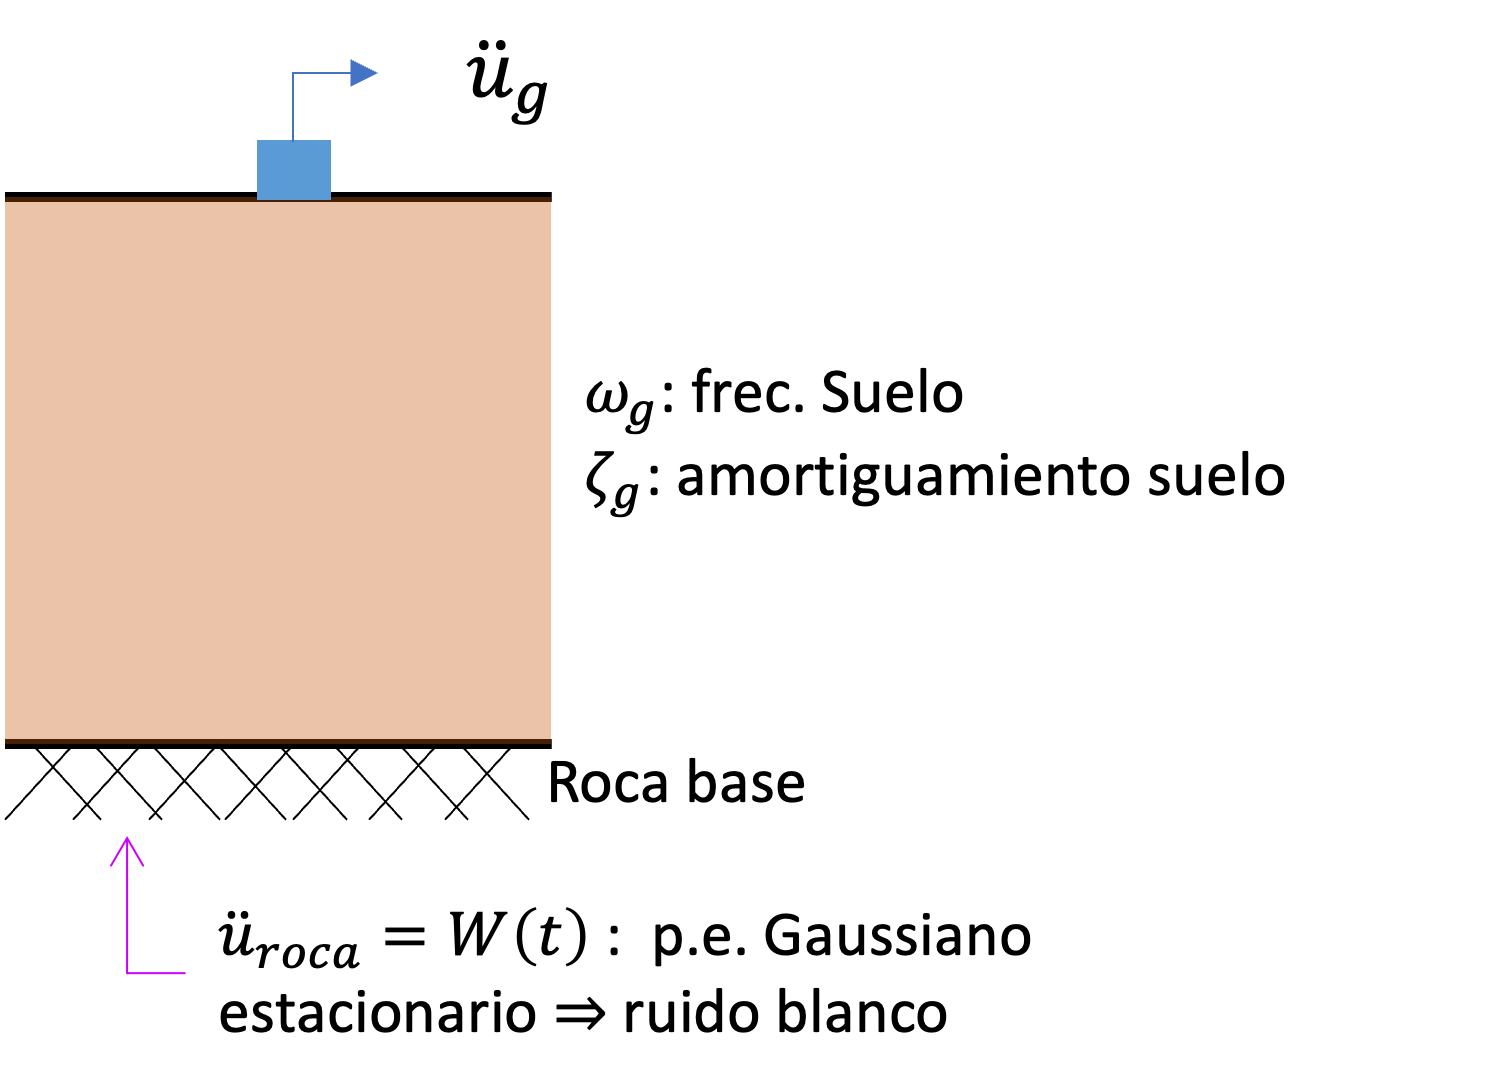
\includegraphics[scale=0.85]{Figuras/KT.png}
\end{figure}
EDM: $a$- estado del suelo
\begin{align*}
    \ddot{a}+2\xi_g\omega_g\dot{a}+\omega_g^2a=W(t) 
\end{align*}

Ruido blanco: 
$$\mathbb{E}\{W(t)\}=0$$ 
$$\mathbb{E}\{W(t)W(t+\tau)\}=2\pi S_0\delta(\tau)$$

$S_0$: poder espectral del sismo en roca (Intensidad del terremoto).\\

\par Ecuación de respuesta:
\begin{align*}
    \ddot{u}_g = -2\xi_g\omega_g \dot{a}-\omega_g^2a
\end{align*}
donde $\ddot{u}_g$ es la aceleración del suelo en campo libre.\\
\par Se puede demostrar que la función de respuesta en frecuencia (FRF) del estado de suelo es:

\begin{align*}
    H_{KT}(\Omega) &= \frac{\omega_g^2+i2\xi_g\omega_g\Omega}{(\omega_g^2-\Omega^2)+i2\xi_g\omega_g\Omega}\\
    |H_{KT}(\Omega)| &= \frac{\omega_g^4+4\xi_g^2\omega_g^2\Omega^2}{(\omega_g^2-\Omega^2)+4\xi_g^2\omega_g^2\Omega^2}
\end{align*}

\begin{figure}[H]
\centering
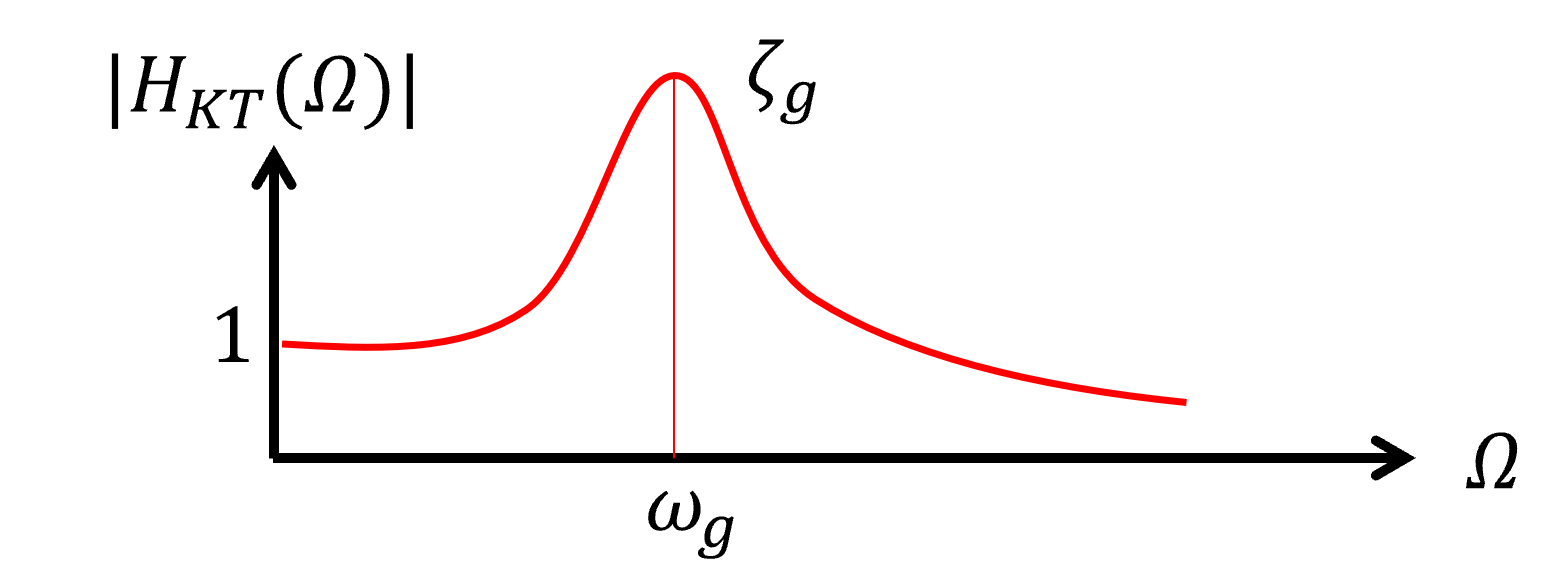
\includegraphics[scale=0.7]{Figuras/HKT.png}
\end{figure}


En espacio-estado:
\begin{align*}
    \dot{x}_g &= A_gx_g+B_gw(t), \quad x_g=a\\
    y_g &= C_gx_g, \quad y_g=\ddot{u}_g
\end{align*}

Diagrama de bloques:

\begin{figure}[H]
\centering
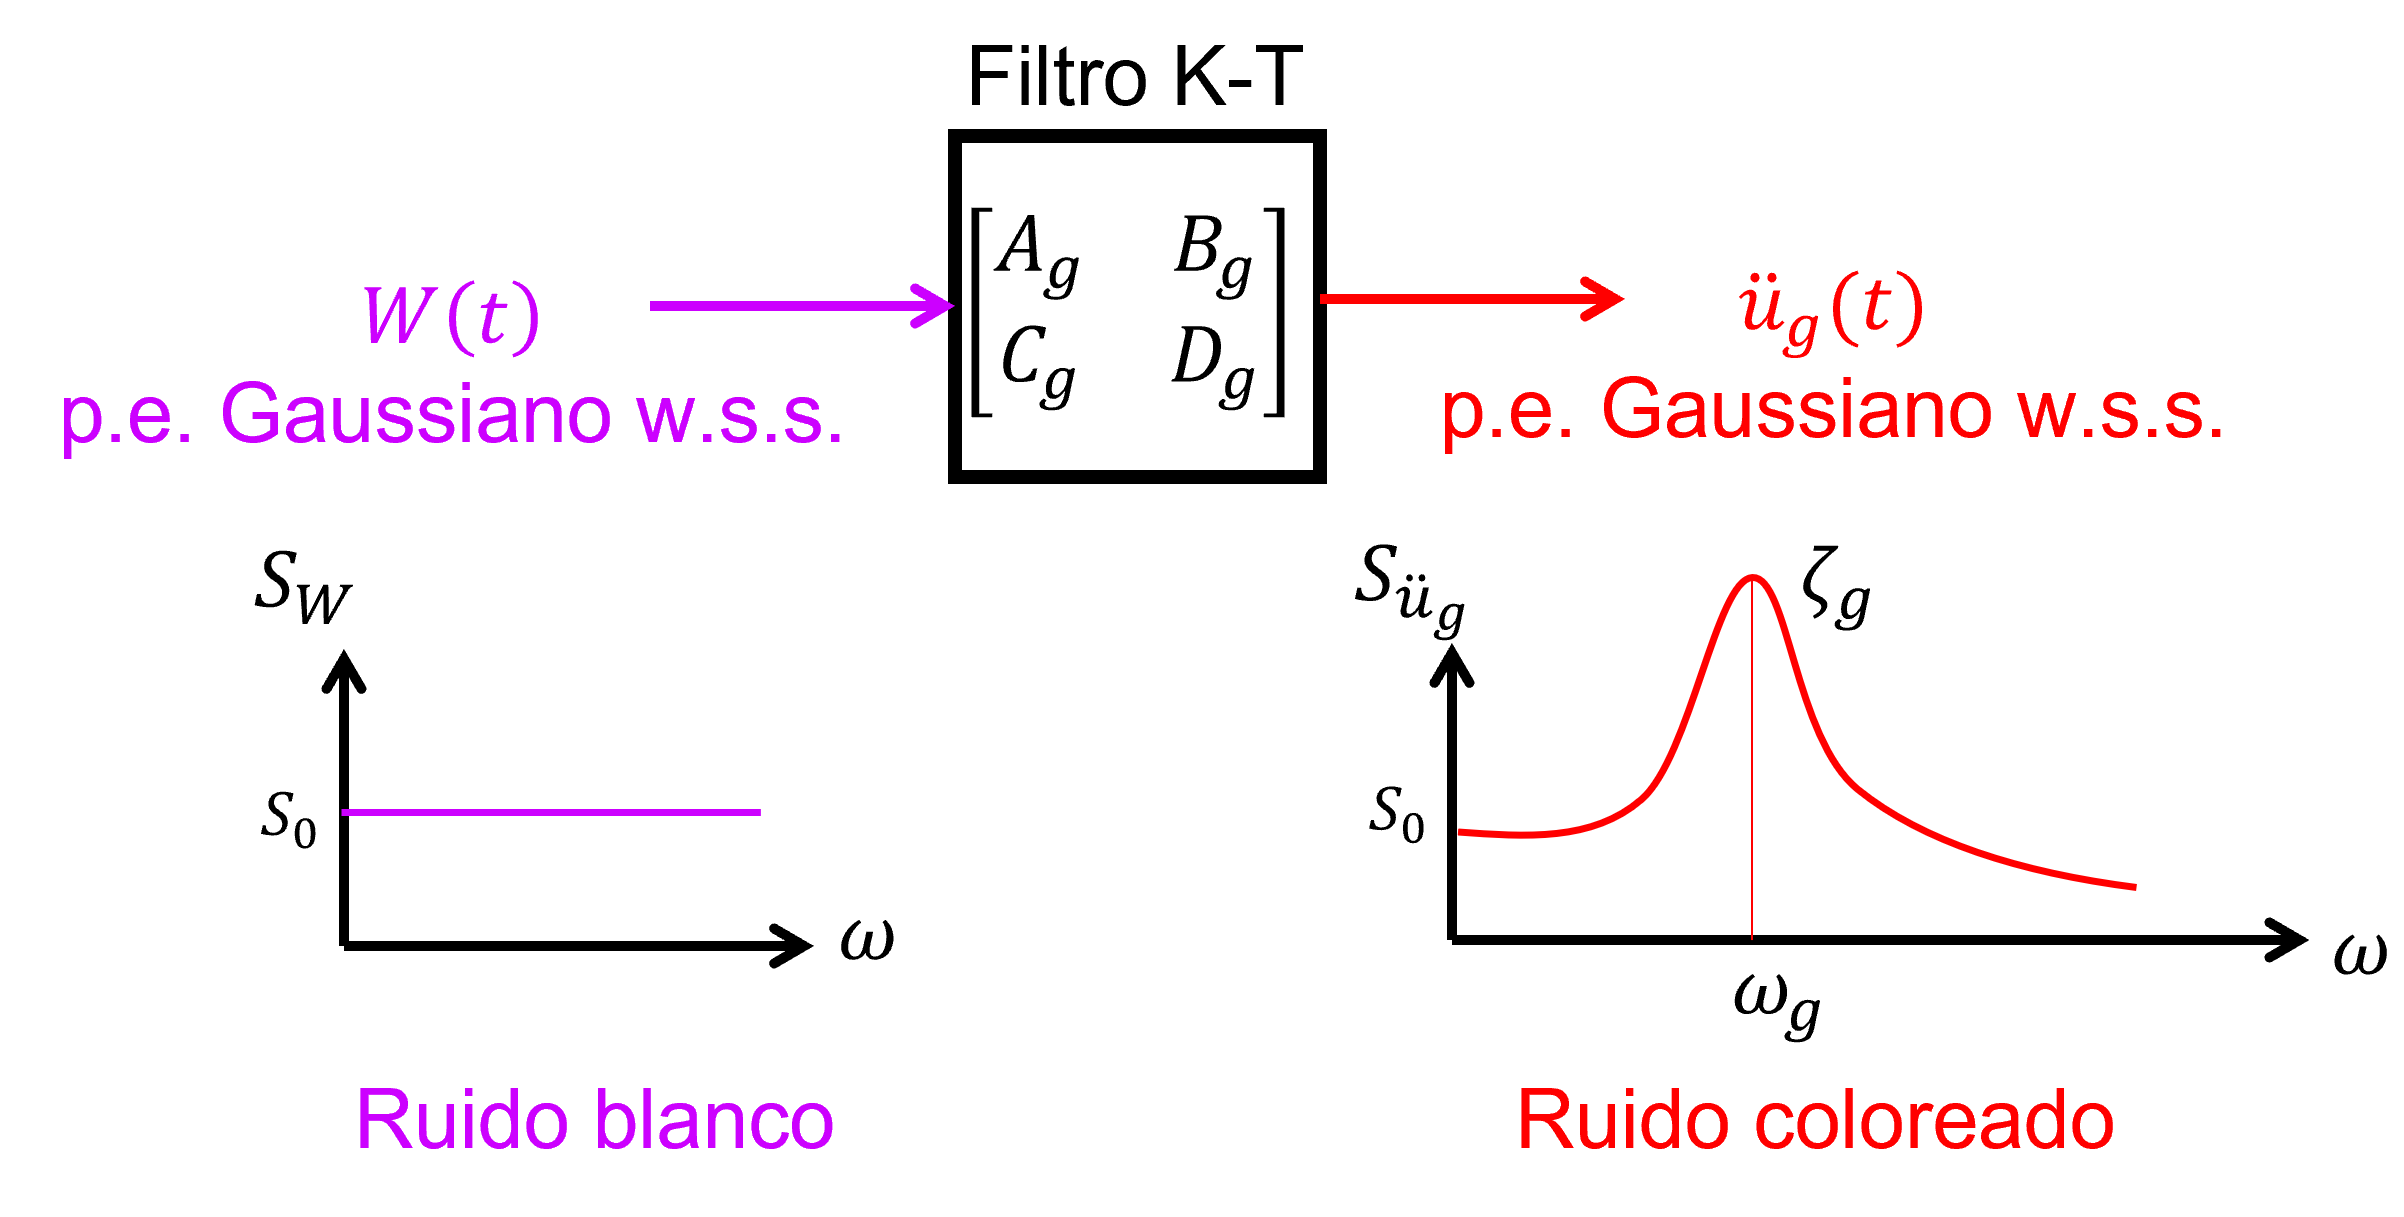
\includegraphics[scale=0.6]{Figuras/diagrama_bloque_KT.png}
\end{figure}

\begin{align*}
    \ddot{u}_g(t) &= h_{KT} \ast W(t)\\
    \ddot{u}_g(t)\ddot{u}_g(t+\tau) &= h_{KT}^2(t) \ast W(t)W(t+\tau)\\
    \Longrightarrow s_{\ddot{u}_g}(\omega) &= |H_{KT}(\omega)|^2s_0
\end{align*}

Parámetros del modelo K-T: $s_0$, $\omega_g$, $\xi_g$.\\
\par Terremoto El Centro (1940): 
\begin{itemize}
    \item $\bar{\omega}_g = 18$ rad/s
    \item $\bar{\xi}_g = 0.60$
    \item $s_0 = $ depende del peak ground acceleration (PGA)
\end{itemize}

En estado estacionario:

\begin{figure}[H]
\centering
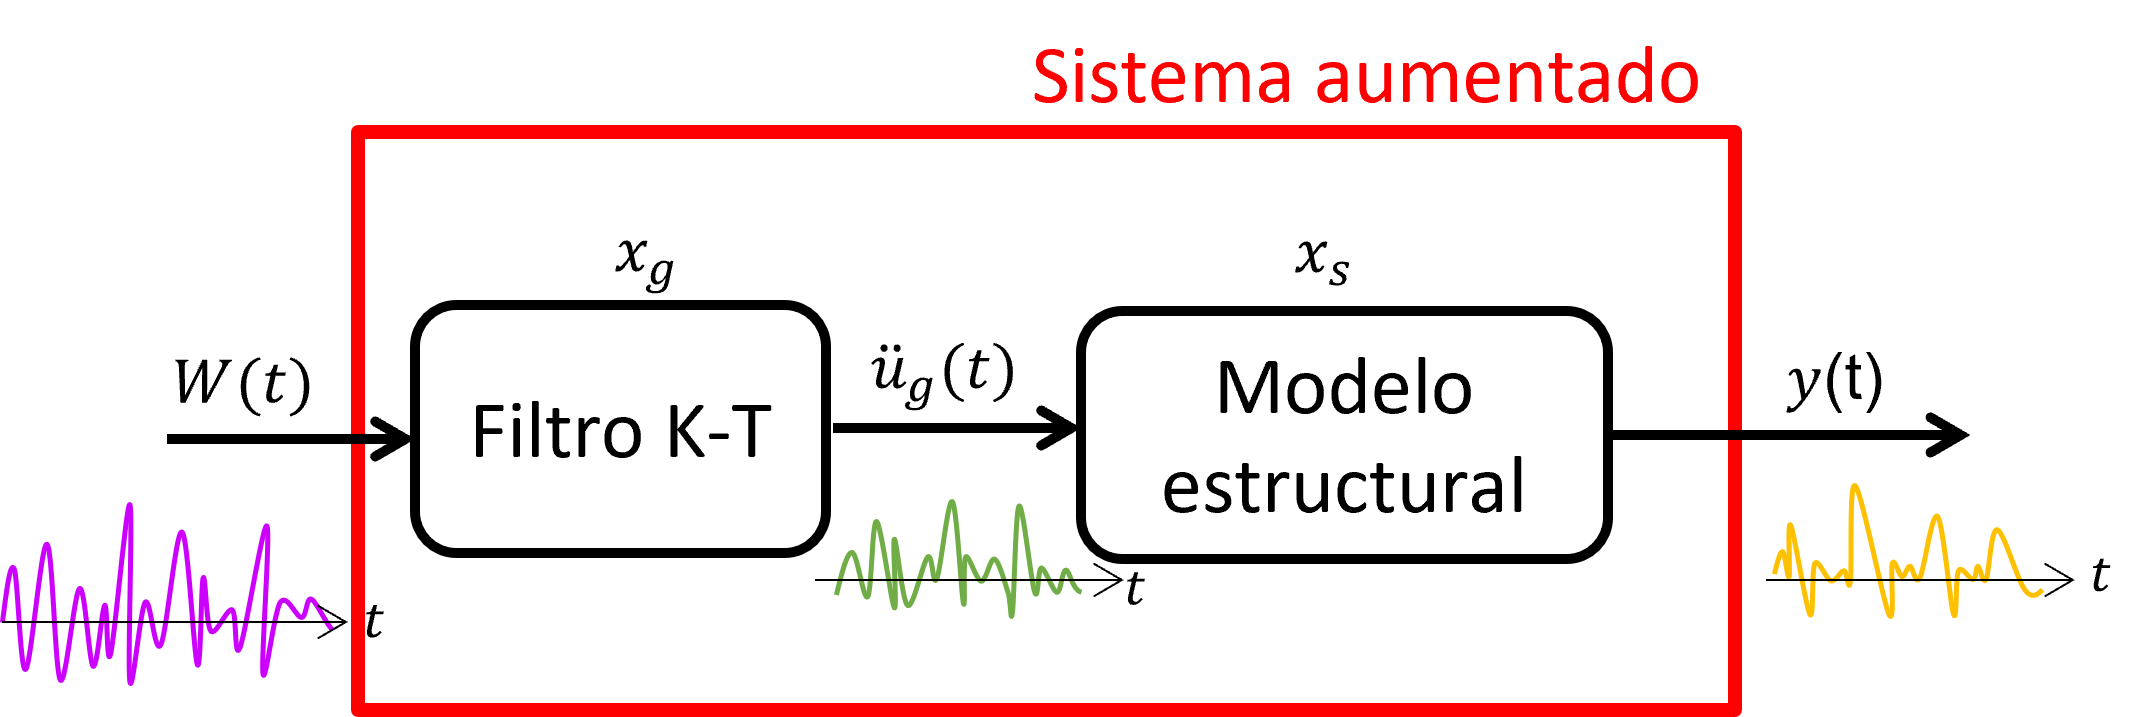
\includegraphics[scale=0.7]{Figuras/estado_estacionario_KT.png}
\end{figure}
Estados: $x_a=\left\{
    \begin{array}{c}
     x_s \\ x_g 
    \end{array}\right\}$
\begin{align*}
    \dot{x}_a&=A_ax_a+B_aW(t)\\
    y &= C_ax_a
\end{align*}

\par Ec. de Lyapunov:
\begin{align*}
    0 &= A_x\Gamma_x +\Gamma_aA_a^\top+Q_a\\
    \Gamma_a &= \mathbb{E}\{x_ax_a^\top\}\\
    \Gamma_y &= C_a\Gamma_aC_a^\top \Longrightarrow \text{RMS respuesta}
\end{align*}

Pero, en realidad los registros sísmicos son p.e. no estacionarios:

\par ¿Podemos ocupar K-T? $\longrightarrow$ Sí, a través de una \textcolor{red}{función de modulación}\\

\begin{figure}[H]
\centering
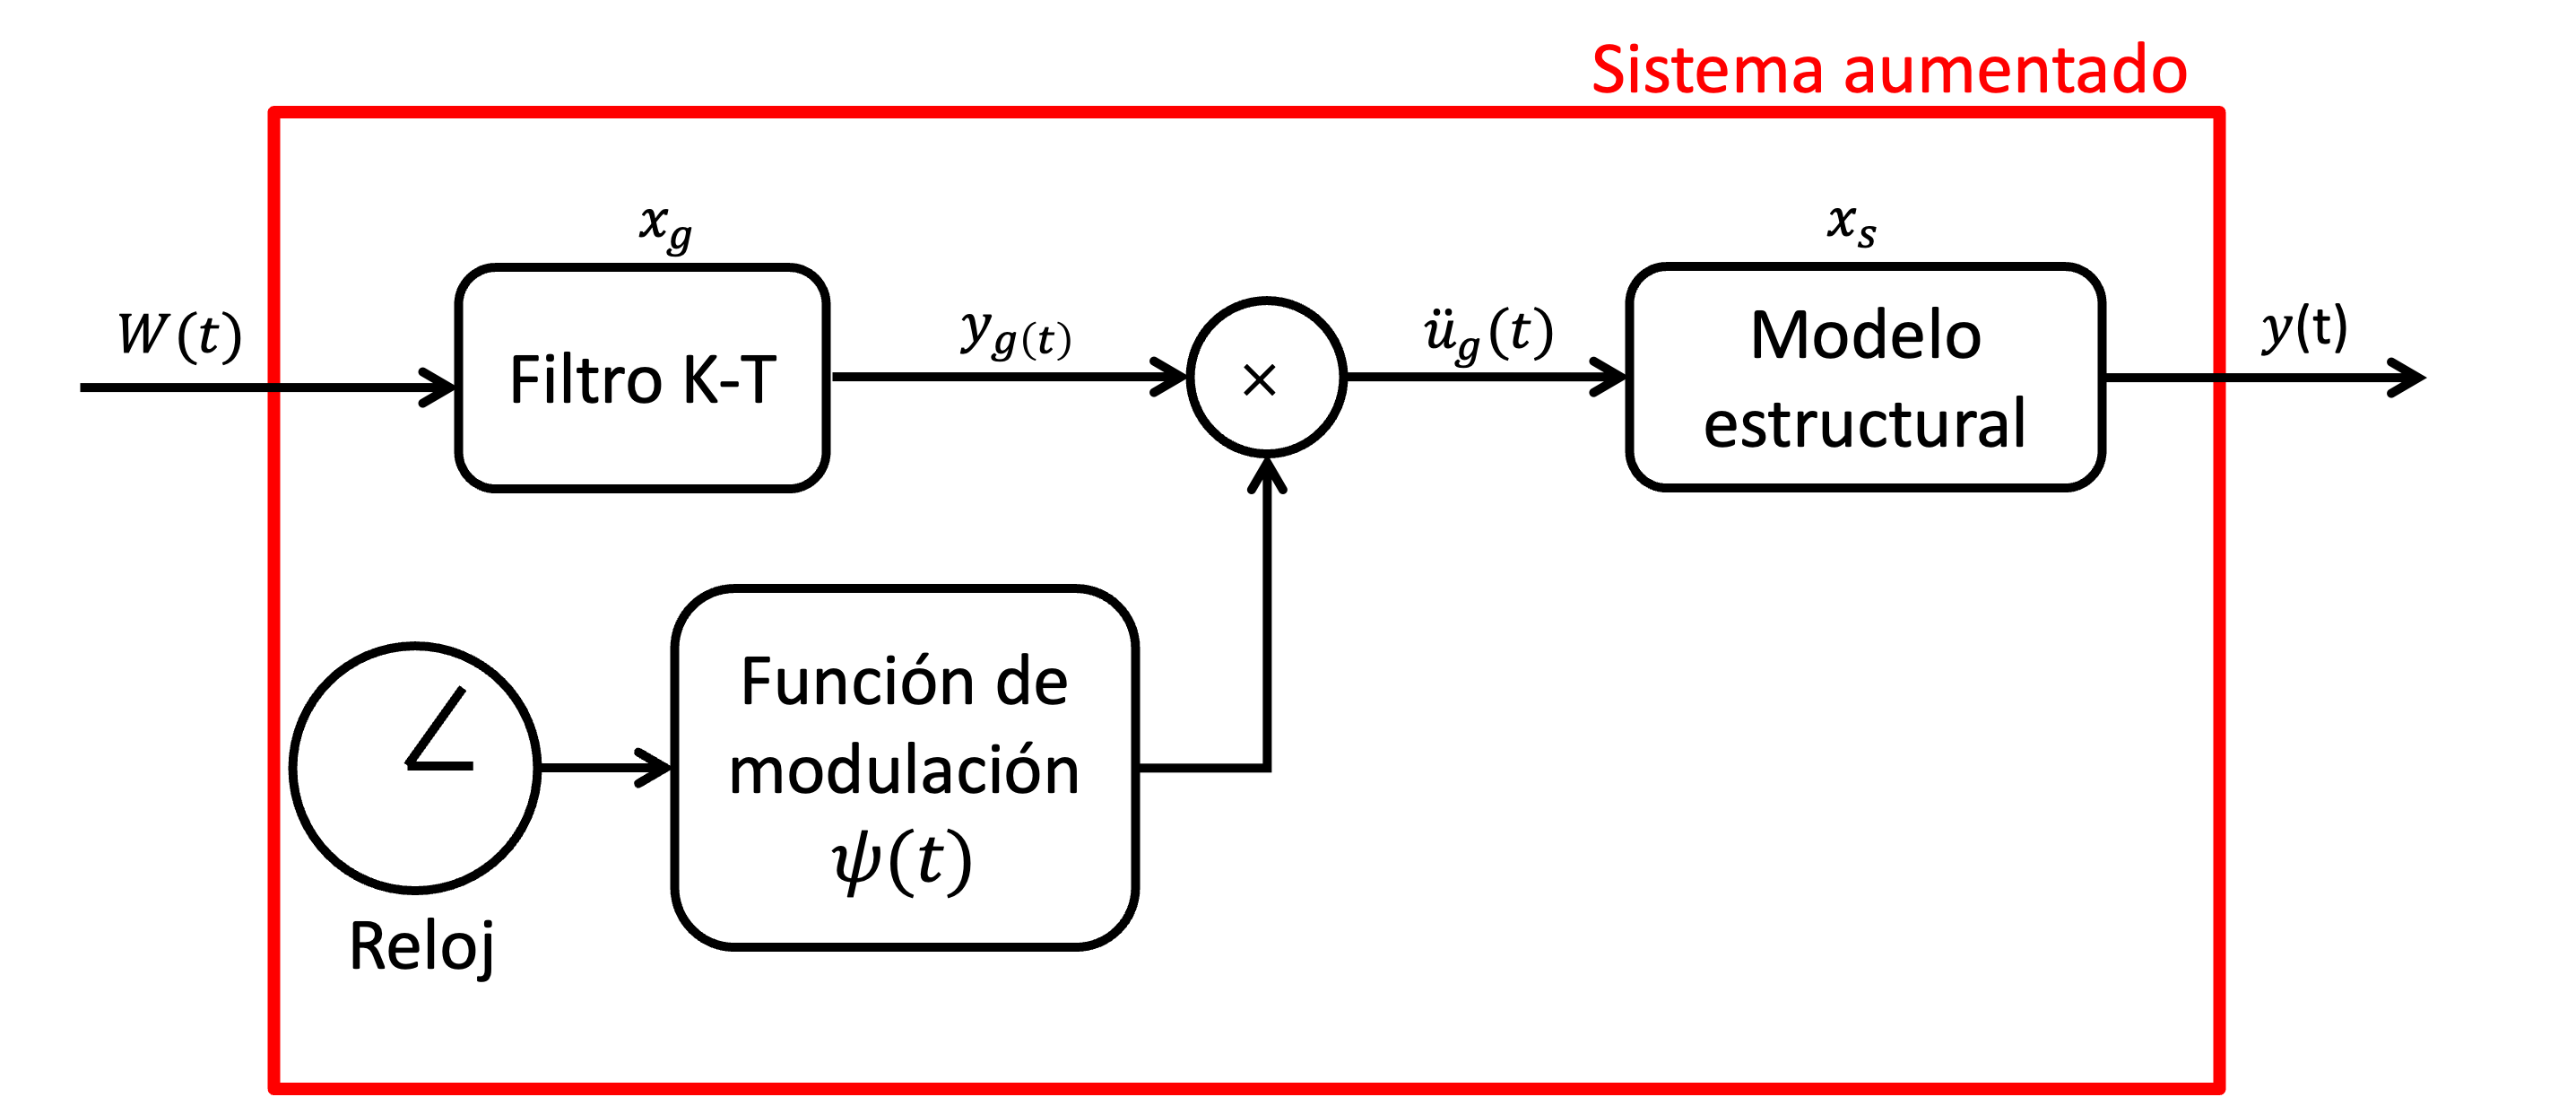
\includegraphics[scale=0.6]{Figuras/func_mod_KT.png}
\end{figure}
\begin{figure}[H]
\centering
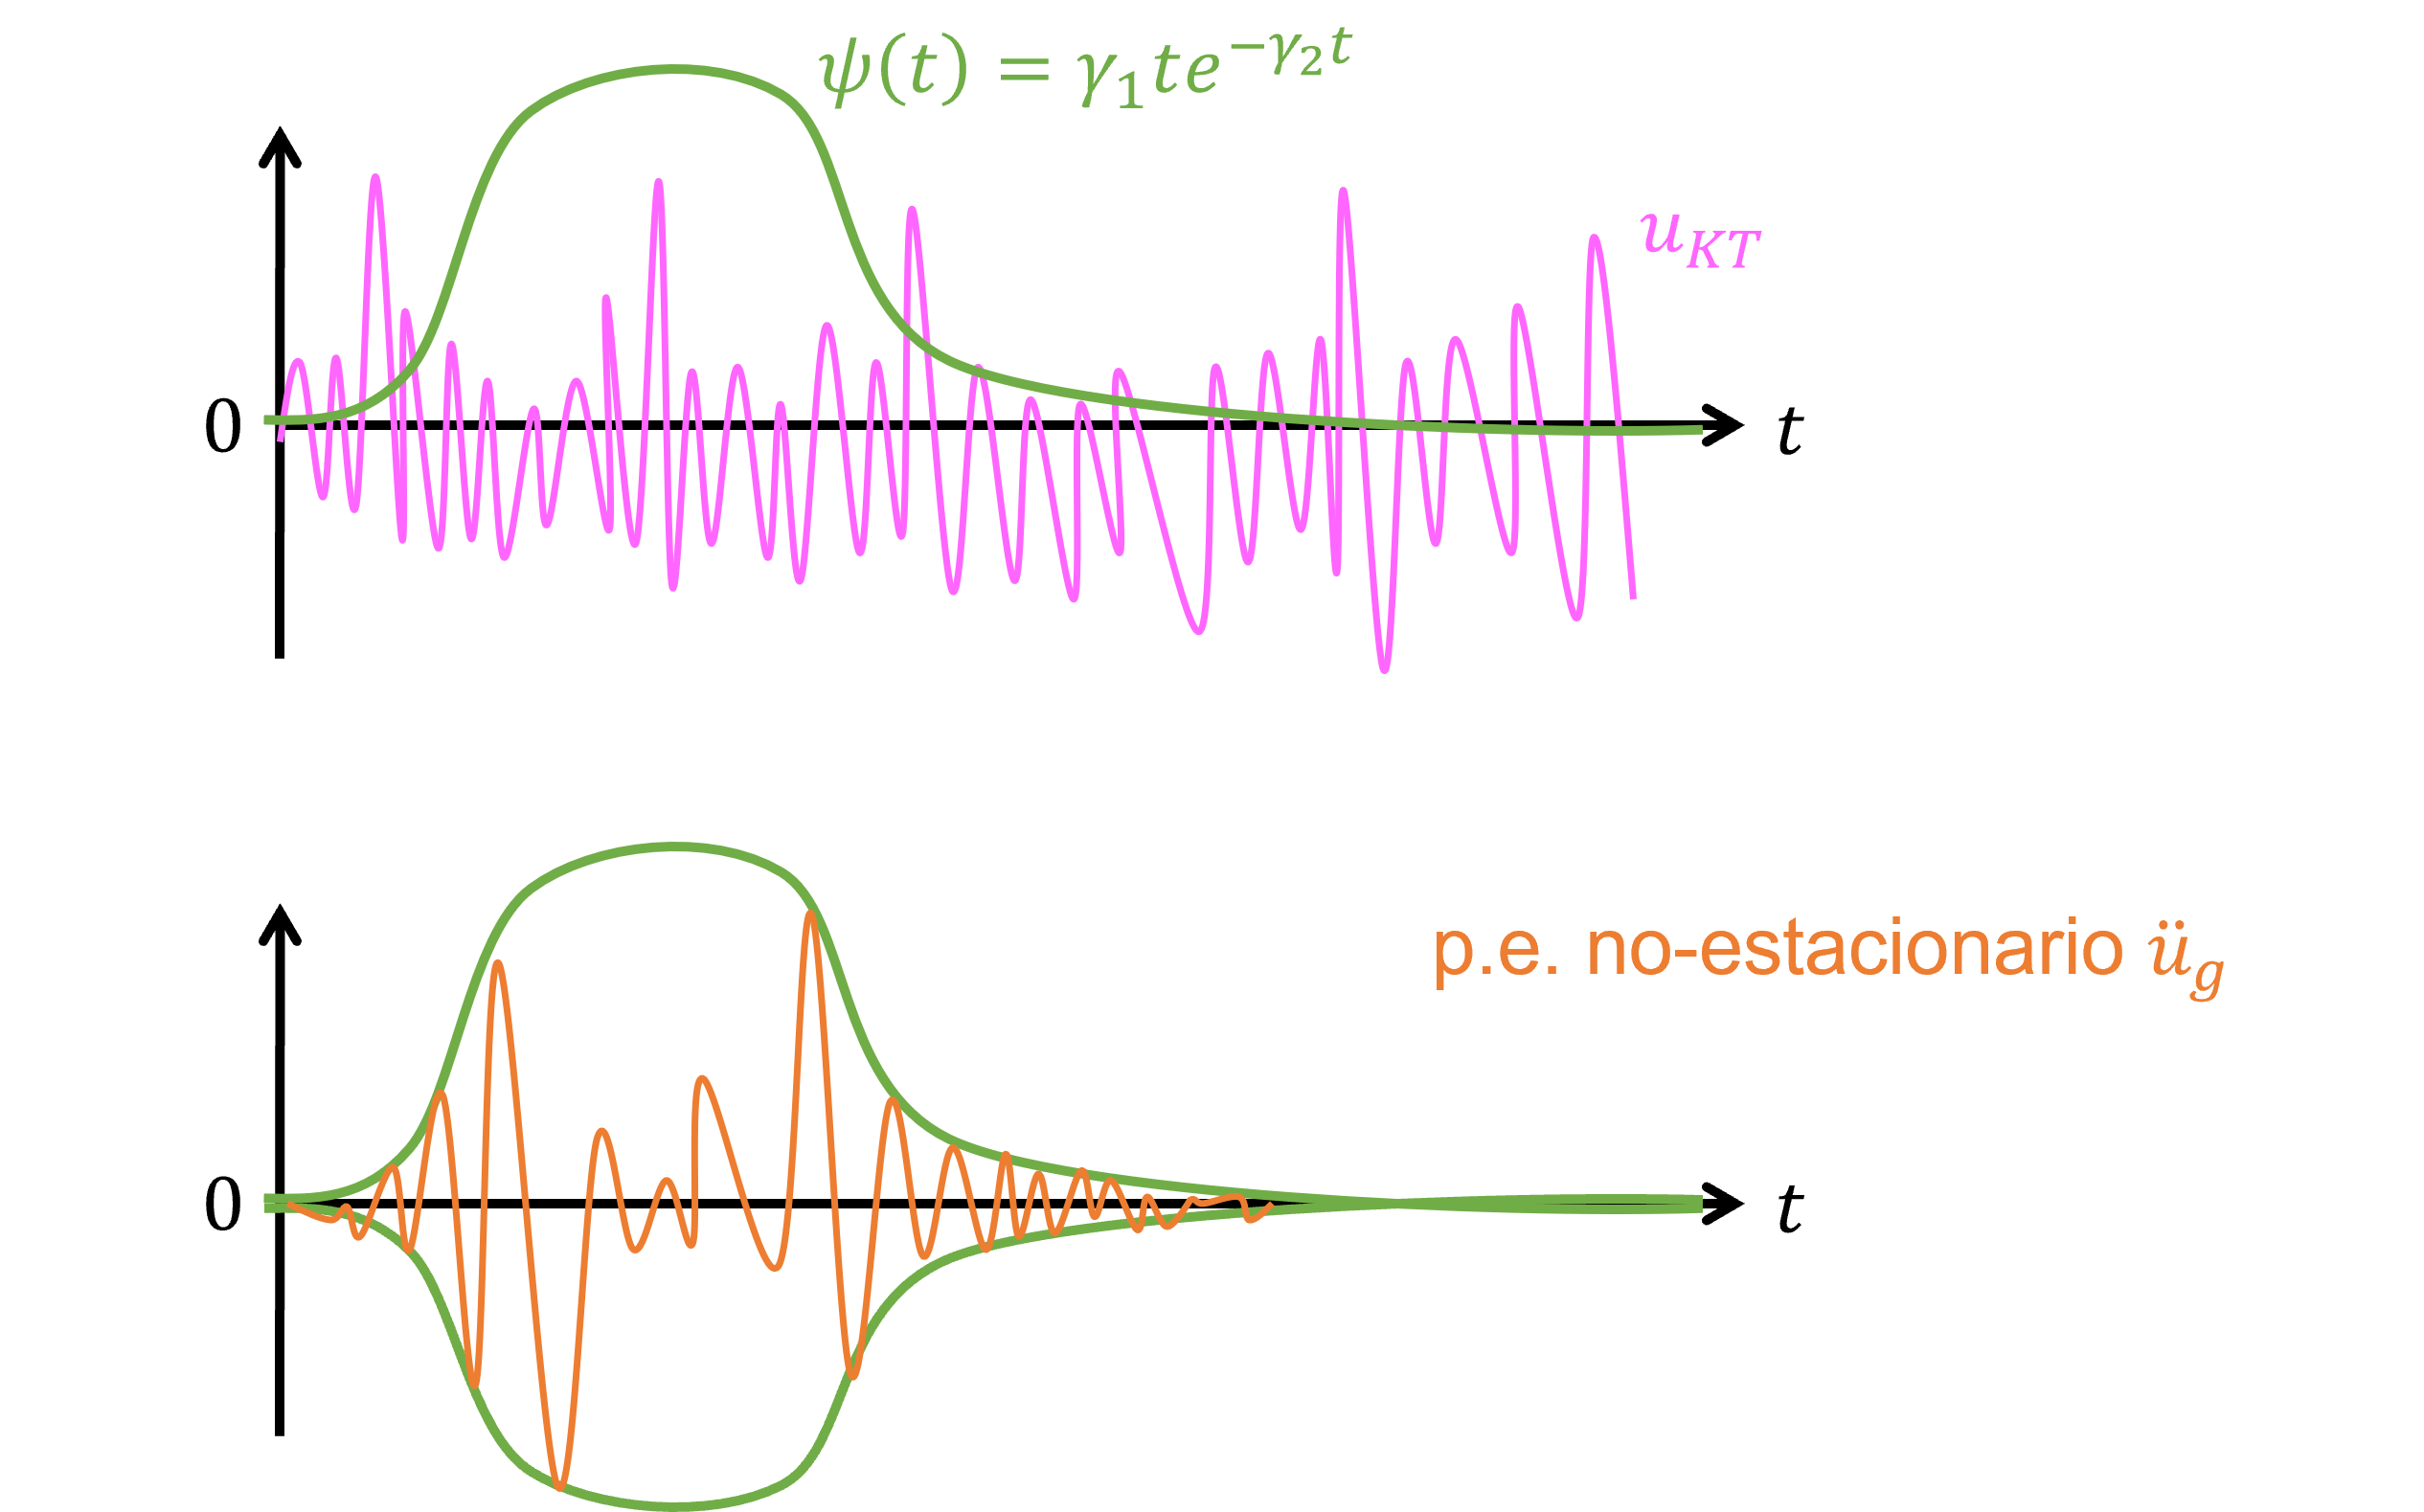
\includegraphics[scale=0.6]{Figuras/func_mod_KT2.png}
\end{figure}

\par Sistema atenuado (LTV): 
\begin{align*}
    \dot{x}_a(t) &= A_a(T)x_a(t)+B_a(t)Z(t)\\
    y(t) &= C_a(t)x_a(t)
\end{align*}
$\Longrightarrow$ Ec. diferencial de Lyapunov:
\begin{align*}
    \dot{\Gamma}_a(t) = A_a(t)\Gamma_a(t)+\Gamma_a(t)A_a^\top (t))+Q_a(t)
\end{align*}

Integrar, resolver $\Gamma_a(T)\Longrightarrow \Gamma_y (t) \Longrightarrow\text{rms } y(t)$.


